\chapter{Analyse}
\label{ch:2}

\section{Anforderungsanalyse}
\label{sec:2.1}

\subsection{Benutzeranforderungen}
Die Applikation erm\"oglicht es dem Benutzer, verschiedene Punkte in ein Koordinatensystem einzutragen und diese durch Interpolation graphisch zu verbinden.\\
\\
Die Applikation gibt dabei zun\"achst ein 100x50 Koordinatensystem auf der X-Y-Ebene vor.\\
Auf der Benutzeroberfl\"ache kann der Benutzer die Gr\"o\ss e des Koordinatensystems, bzw. den Definitionsbereich ver\"andern.\\
Mit der linken Maustaste kann der Benutzer Punkte im abgebildeten Koordinatensystem auf der Zeichenfl\"ache einzeichnen und mit einem rechten Mausklick auf einen Punkt kann der Benutzer diesen l\"oschen.
Ist mehr als ein Punkt in dem angeklickten L\"oschradius, so l\"oscht die Applikation den Punkt mit dem kleinsten x-Wert.\\
Sind mindestens zwei Punkte eingezeichnet, nachdem ein Punkt hinzugef\"ugt oder gel\"oscht wurde, dann startet die Applikation automatisch die Interpolation und verbindet die eingezeichneten Punkte auf der Zeichenfl\"ache mithilfe der gew\"ahlten Interpolationsmethode.\\
Der Benutzer kann auf einer Auswahlbox auf der Benutzeroberfl\"ache zwischen einer Interpolation durch ein Polynom (Grad m-1 bei m zu Interpolierenden Punkten), oder durch lineare oder kubische Splines w\"ahlen.\\
Nach dem Start des Programmes oder nach dem Zur\"ucksetzen ist die Interpolationsart standardm\"a\ss ig auf lineare Splines eingestellt.\\
Der Benutzer kann zu jeder Zeit  mit dem Button "'Reset"  das leere 100x50 Koordinatensystem mit den Standardeinstellungen wiederherstellen oder mit dem Button "'Beenden" das Programm beenden. \\
\\
\subsection{Anwendungsfallanalyse}

\textbf{Anwendungsfalldiagramm:}

\begin{figure}[H]
\centering
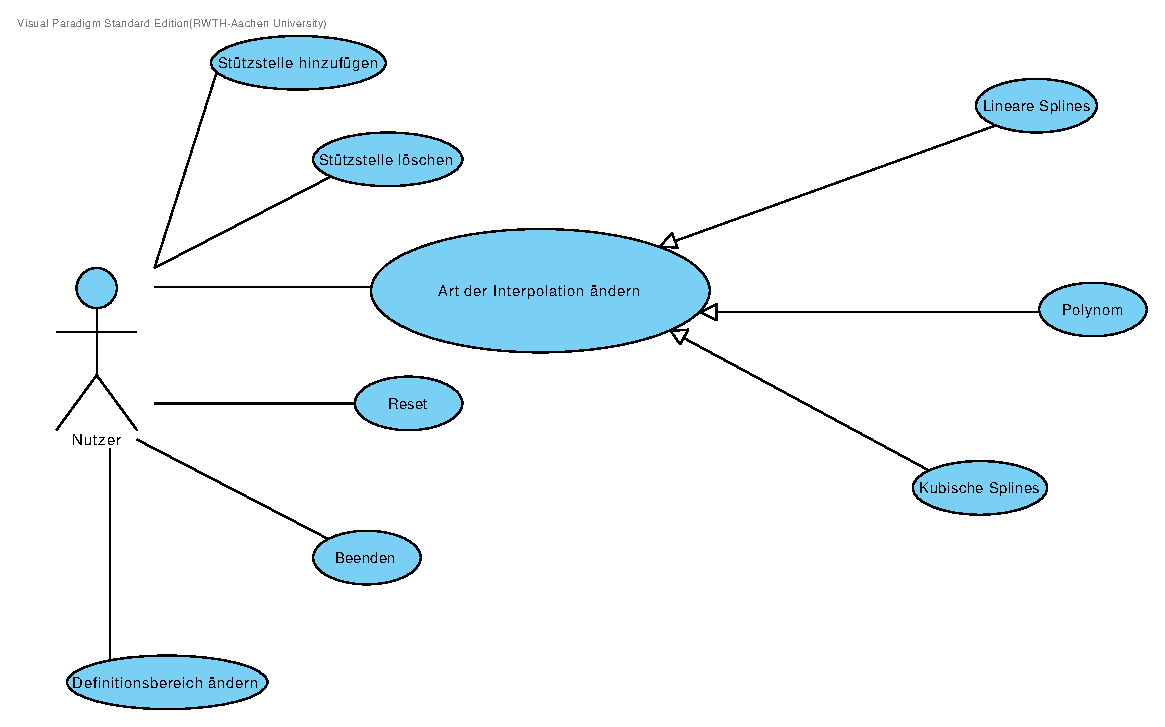
\includegraphics[width=\textwidth]{Aktivitaetsdiagramm/Top_Level_Use_Cases}
\caption{Anwendungsfalldiagramm}
\label{fig:Anwendungsfalldiagramm}
\end{figure}

\textbf{Aktivit\"atsdiagramme:}

\textbf{Art der Interpolation \"andern}
  \begin{itemize}
  \item \textit{Ziel:} Der Nutzer will die Interpolationsart \"andern.
  \item \textit{Einordnung:} Hauptfunktion
  \item \textit{Vorbedingung:} Die Applikation ist ge\"offnet und zeigt die Zeichenfl\"ache sowie die Benutzeroberfl\"ache an.
  \item \textit{Nachbedingung:} Die Applikation zeigt die neu berechnete Kurve auf der Zeichenfl\"ache an.
  \item \textit{Nachbedingung im Fehlerfall:} 
  \item \textit{Hauptakteure:} Nutzer
  \item \textit{Nebenakteure:} 
  \item \textit{Ausl\"oser:} Der Nutzer will die Interpolationsart \"andern.
  \item \textit{Standardablauf:}
    \begin{enumerate}[label=(\arabic*)]
    \item Der Nutzer klickt mit der linken Maustaste auf die Auswahlbox mit der \"Uberschrift "'Interpolationsart", welche sich auf der Benutzeroberfl\"ache befindet.
    \item Die Applikation zeigt alle m\"oglichen Interpolationsmethoden in der Auswahlbox an.
    \item Der Nutzer w\"ahlt mit der linken Maustaste eine Interpolationsart aus.
    \item Die Applikation f\"uhrt die Interpolation mit der ausgew\"ahlten Interpolationsmethode aus.
    \item Die Applikation zeigt die neu berechnete Interpolation auf der Zeichenfl\"ache an.
    \end{enumerate}
  \end{itemize}

\begin{figure}[H]
\centering
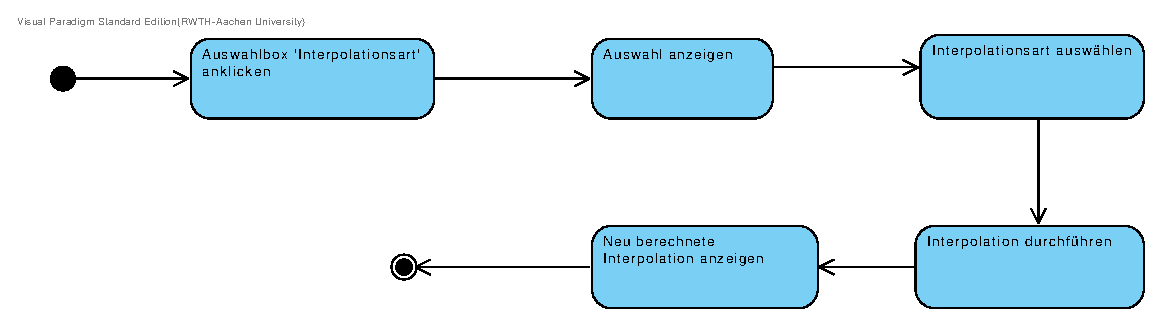
\includegraphics[width=\textwidth]{Aktivitaetsdiagramm/interpolationAuswaehlen.eps}
\caption{Interpolationsart aendern}
\label{fig:Interpolationsart aendern}
\end{figure}

\hfill \\
\hfill \\
\textbf{Reset}
  \begin{itemize}
  \item \textit{Ziel:} Es sollen alle St\"utzstellen und die Kurve von der Zeichenfl\"ache gel\"oscht, sowie der Definitionsbereich und die Interpolationsart auf den Defaultmodus (Lineare Spline Interpolation ([0,100]x[0,50]) zur\"uckgesetzt werden.
  \item \textit{Einordnung:} Hauptfunktion
  \item \textit{Vorbedingung:} Die Applikation ist ge\"offnet und zeigt die Zeichenfl\"ache sowie die Benutzeroberfl\"ache an.
  \item \textit{Nachbedingung:} Die Applikation hat alle St\"utzstellen auf der Zeichenfl\"ache gel\"oscht und der Definitionsbereich sowie die Interpolationsart sind im Defaultmodus.
  \item \textit{Nachbedingung im Fehlerfall:} 
  \item \textit{Hauptakteure:} Nutzer
  \item \textit{Nebenakteure:}
  \item \textit{Ausl\"oser:} Der Nutzer m\"ochte die Applikation auf den Defaultmodus zur\"ucksetzen.
  \item \textit{Standardablauf:}
    \begin{enumerate}[label=(\arabic*)]
    \item Der Nutzer klickt mit der linken Maustaste auf den Button 'Reset', welcher sich auf der Benutzeroberfl\"ache befindet.
    \item Die Applikation stellt den Defaultmodus wieder her und l\"oscht die St\"utzstellen.
   % \item Die Applikation entfernt alle St\"utzstellen.							%Sollen die Aktivit\"aten des Systemes angezeigt werden?
    %\item Die Applikation ruft den UC Case Interpolieren auf
   %\item Die Applikation setzt den Definitionsbereich auf [0,50]x[0,100].
  %  \item Die Applikation setzt die Interpolationsart auf  'Lineare Splines'.
    
    \end{enumerate}
 \end{itemize}  
\begin{figure}[H]
\centering
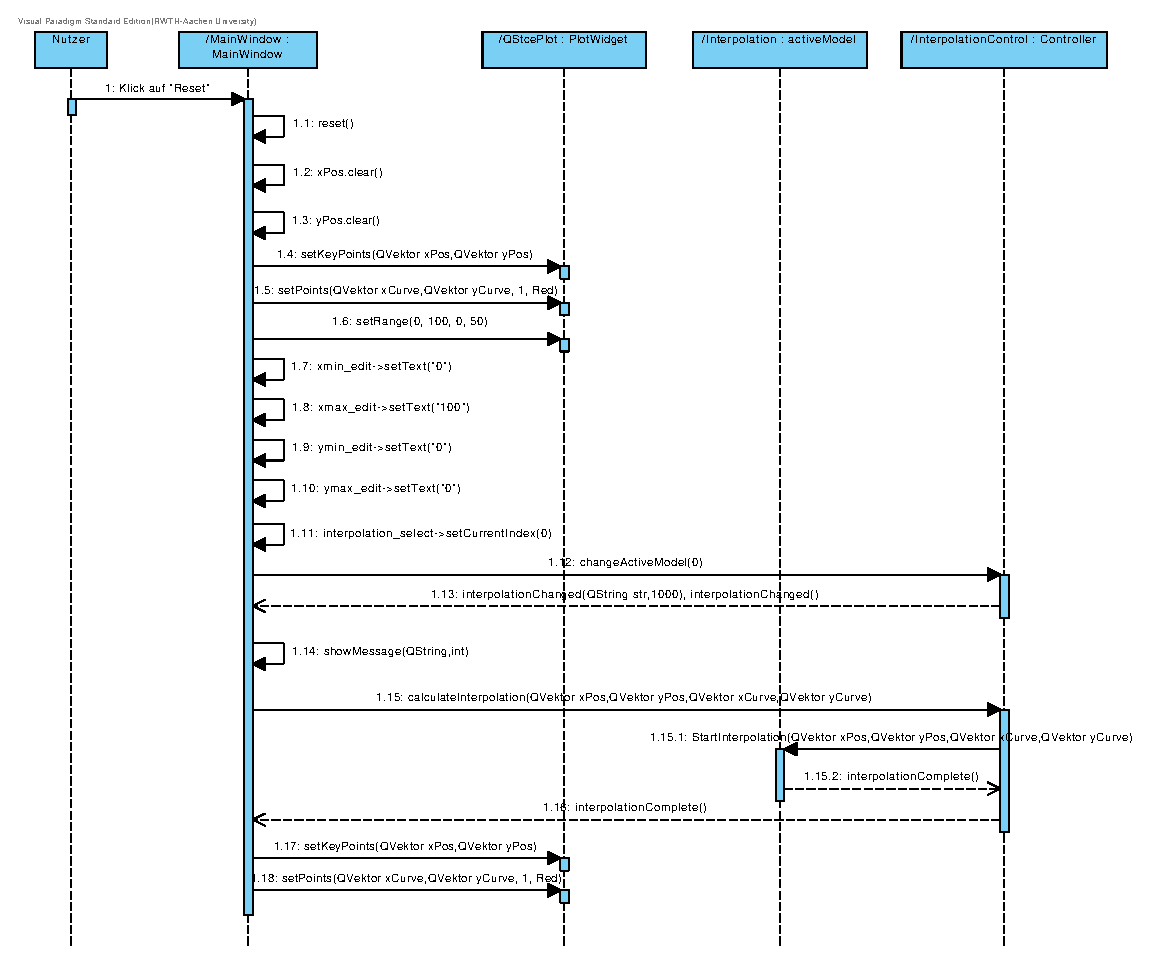
\includegraphics[width=\textwidth]{Aktivitaetsdiagramm/Reset.eps}
\caption{Reset}
\label{fig:Reset}
\end{figure}

\hfill \\
\hfill \\
\textbf{Definitionsbereich \"andern}
  \begin{itemize}
  \item \textit{Ziel:} Der Definitionsbereich soll ge\"andert werden
  \item \textit{Einordnung:}  Hauptfunktion
  \item \textit{Vorbedingung:} Die Applikation ist ge\"offnet und zeigt die Zeichenfl\"ache sowie die Benutzeroberfl\"ache an.
  \item \textit{Nachbedingung:} Die Applikation zeigt die aktualisierte Zeichenfl\"ache sowie Benutzeroberfl\"ache mit den neuen Grenzen an.
  \item \textit{Nachbedingung im Fehlerfall:} Die Applikation zeigt eine Fehlermeldung an und ver\"andert die Zeichenfl\"ache nicht.
  \item \textit{Hauptakteure:} Nutzer
  \item \textit{Nebenakteure:}
  \item \textit{Ausl\"oser:} Der Nutzer will den Definitionsbereich \"andern
  \item \textit{Standardablauf:}
    \begin{enumerate}[label=(\arabic*)]
    \item Der Nutzer klickt mit der linken Maustaste auf eins der Textfelder auf der Benutzeroberfl\"ache unter der \"Uberschrift "'Definitionsbereich".
    \item Der Nutzer \"andert den Wert im Textfeld.
    \item Der Nutzer bet\"atigt mit der linken Maustaste den Button 'Definitionsbereich setzen'.
    \item Die Applikation pr\"uft, ob Zahlen eingegeben wurden.
    \item Die Applikation pr\"uft, ob $ x_{min} > x_{max}$ ist. 
    \item Die Applikation pr\"uft, ob $ y_{min} > y_{max}$ ist.
    \item Die Applikation \"andert den Definitionsbereich auf die gew\"unschten Werte.
    \end{enumerate}
      \item \textit{Verzweigungen:}
     \begin{enumerate}[label=(2a\arabic*)]            	\setcounter{enumii}{3}
      \item Der Nutzer will noch einen anderen Wert des Definitionsbereiches \"andern.
   	\item Der Nutzer geht zu Schritt '1' zur\"uck.
                \end{enumerate}      
    \begin{enumerate}[label=(4a\arabic*)]
      \item Der Nutzer hat eine ung\"ultige Eingabe get\"atigt.
      \item Die Applikation gibt eine Fehlermeldung aus.
      \end{enumerate}
                      \begin{enumerate}[label=(5a\arabic*)]
    \setcounter{enumii}{4}
    \item Die Applikation erkennt, dass  '$ x_{min} > x_{max}$'  ist.
      \item Die Applikation gibt eine Fehlermeldung aus.
      \end{enumerate}
           \begin{enumerate}[label=(6a\arabic*)]
     \setcounter{enumii}{5}
    \item Die Applikation erkennt, dass  '$ y_{min} > y_{max}$'  ist.
    \item Die Applikation gibt eine Fehlermeldung aus.
      \end{enumerate}
  \end{itemize}

\begin{figure}[H]
\centering
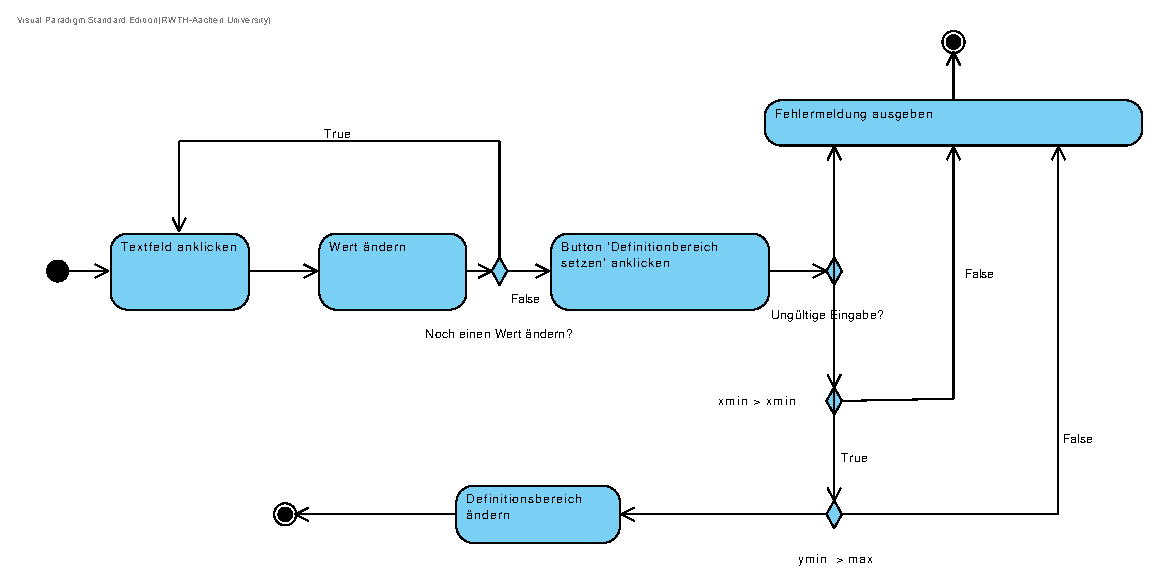
\includegraphics[width=\textwidth]{Aktivitaetsdiagramm/definitionbereichAendern.eps}
\caption{Definitionsbereich aendern}
\label{fig:Definitionsbereich aendern}
\end{figure}

\hfill \\
\hfill \\
\textbf{Beenden}
  \begin{itemize}
  \item \textit{Ziel:} Die Applikation soll beendet werden
  \item \textit{Einordnung:} Hauptfunktion
  \item \textit{Vorbedingung:} Die Applikation ist ge\"offnet und zeigt die Zeichenfl\"ache sowie die Benutzeroberfl\"ache an.
  \item \textit{Nachbedingung:} Die Applikation wurde erfolgreich beendet.
  \item \textit{Nachbedingung im Fehlerfall:} 
  \item \textit{Hauptakteure:} Nutzer
  \item \textit{Nebenakteure:}
  \item \textit{Ausl\"oser:} Der Nutzer m\"ochte die Applikation beenden.
    \item \textit{Standardablauf:}
    \begin{enumerate}[label=(\arabic*)]
    \item Der Nutzer bet\"atigt auf der Benutzeroberfl\"ache mit der linken Maustaste den Button 'Beenden'.
    \item Die Applikation schlie\ss t.
    \end{enumerate}
 \end{itemize}  
\begin{figure}[H]
\centering
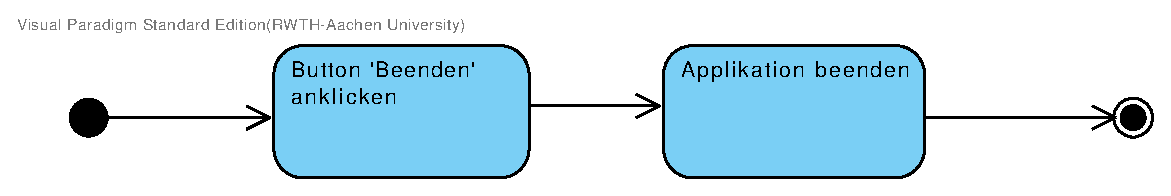
\includegraphics[width=\textwidth]{Aktivitaetsdiagramm/beenden.eps}
\caption{Beenden}
\label{fig:Beenden}
\end{figure}

\hfill \\
\hfill \\
\textbf{St\"utzstelle l\"oschen}
  \begin{itemize}
  \item \textit{Ziel:} Es soll eine vom Nutzer angeklickte St\"utzstelle von der Zeichenfl\"ache gel\"oscht werden.
  \item \textit{Einordnung:} Hauptfunktion
  \item \textit{Vorbedingung:} Die Applikation ist ge\"offnet und zeigt die Zeichenfl\"ache sowie die Benutzeroberfl\"ache an.
  \item \textit{Nachbedingung:} Die Applikation zeigt die neu berechnete Interpolation ohne die gel\"oschte St\"utzstelle auf der Zeichenfl\"ache an.
  \item \textit{Nachbedingung im Fehlerfall:}  Die Applikation zeigt die urspr\"ungliche Interpolation an.
  \item \textit{Hauptakteure:} Nutzer
  \item \textit{Nebenakteure:} 
  \item \textit{Ausl\"oser:} Der Nutzer m\"ochte eine St\"utzstelle von der Zeichenfl\"ache l\"oschen
  \item \textit{Standardablauf:}
    \begin{enumerate}[label=(\arabic*)]
    \item Der Nutzer klickt mit der rechten Maustaste auf eine beliebige Stelle der Zeichenfl\"ache.
    \item Die Applikation l\"oscht die im L\"oschradius befindliche St\"utzstelle mit dem kleinsten x-Wert.
    \item Die Applikation f\"uhrt die Interpolation mit den verbleibenden St\"utzstellen aus.
    \item Die Applikation zeigt die neu berechnete Interpolation auf der Zeichenfl\"ache an.
   
    \end{enumerate}
  \item \textit{Verzweigungen:}
    \begin{enumerate}[label=(\arabic*a)]
    \setcounter{enumii}{1}
      \item Die Applikation kann keine St\"utzstelle im L\"oschradius identifizieren.
      \item Der Use Case wird beendet.
      \end{enumerate}

 \end{itemize}

\begin{figure}[H]
\centering
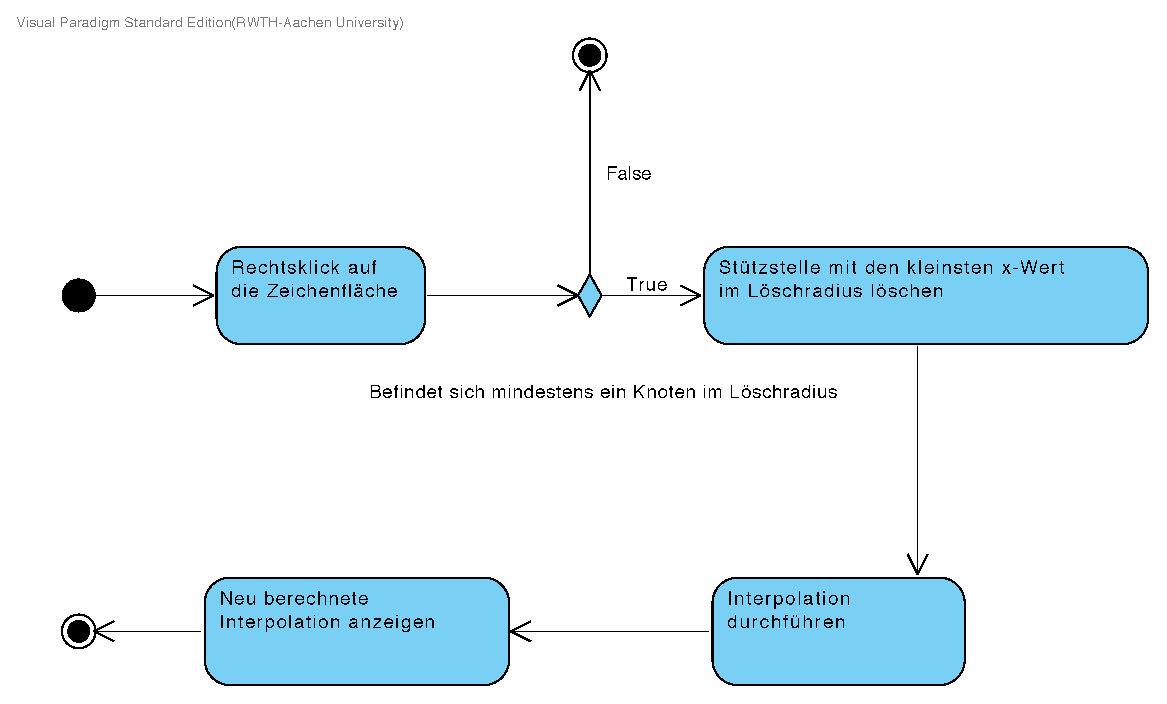
\includegraphics[width=\textwidth]{Aktivitaetsdiagramm/stuetzstelleLoeschen.eps}
\caption{Stuetzstelle loeschen}
\label{fig:Stutzstelle loeschen}
\end{figure}

\hfill \\
\hfill \\
\textbf{St\"utzstelle hinzuf\"ugen}
  \begin{itemize}
  	\item \textit{Ziel:} Die Interpolation soll um eine St\"utzstelle erweitert werden.
  	\item \textit{Einordnung:} Hauptfunktion
  	\item \textit{Vorbedingung:} Die Applikation ist ge\"offnet und zeigt die Zeichenfl\"ache sowie die Benutzeroberfl\"ache an.
  	\item \textit{Nachbedingung:} Die Applikation zeigt die neu berechnete Interpolation mit der hinzugef\"ugten St\"utzstelle auf der Zeichenfl\"ache an.
  \item \textit{Nachbedingung im Fehlerfall:} 
  \item \textit{Hauptakteure:} Nutzer
  \item \textit{Nebenakteure:} 
  \item \textit{Ausl\"oser:} Der Nutzer m\"ochte eine St\"utzstelle auf der Zeichenfl\"ache hinzuf\"ugen.
  \item \textit{Standardablauf:}
    \begin{enumerate}[label=(\arabic*)]
    \item Der Nutzer klickt mit der linken Maustaste auf eine beliebige Stelle der Zeichenfl\"ache.
    \item Die Applikation erzeugt eine St\"utzstelle auf dem angeklickten Punkt.
    \item Die Applikation f\"uhrt die Interpolation mit den neuen St\"utzstellen aus.
    \item Die Applikation zeigt die neu berechnete Interpolation auf der Zeichenfl\"ache an.
    \end{enumerate}
  \end{itemize}

\begin{figure}[H]
\centering
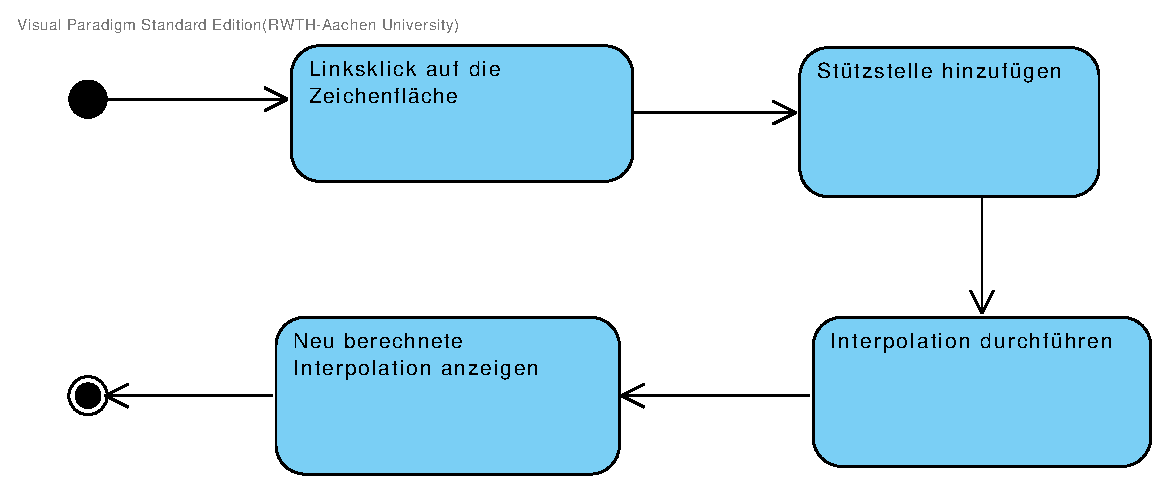
\includegraphics[width=\textwidth]{Aktivitaetsdiagramm/stutzstelleHInzufuegen.eps}
\caption{Stuetzstelle hinzufuegen}
\label{fig:Stuetzstelle hinzufuegen}
\end{figure}



\section{Systemanforderungen}

\subsection{Funktionale Anforderung}
\begin{itemize}
\item Anzeigen einer Zeichenfl\"ache
\item Anzeigen einer Benutzeroberfl\"ache, welche folgende Funktionen bereitstellt:
	\begin{enumerate}
	\item Auswahl der Interpolationmethode
	\item \"Anderung des Definitionsbereichs
	\item Zur\"ucksetzten der Zeichenfl\"ache und Einstellungen auf default
	\item Beenden Button
	\end{enumerate}
\item Anzeigen von Fehlermeldungen
\item Eingabe von Gleitkommazahlen 
\item Anzeigen einer Interpolationskurve
\item Darstellung von Punkten auf der Zeichenfl\"ache
\item Speichern der Punkte (Gleitkommazahlen, ganze Zahlen)
\item L\"oschen und Hinzuf\"ugen von Punkten
\item Test auf G\"ultigkeit des Definitionsbereichs
\item Anzeigen von Gleitkommazahlen auf 2 Nachkommastellen 
\item Nach dem Starten des Programms werden Defintionsbereich und Interpolationsart standardm\"a\ss ig fesgelegt
\end{itemize}
\subsection{Nicht Funktionale Anforderung}
\begin{itemize}
\item Hinzuf\"ugen und L\"oschen der Punkte durch Mausklick m\"oglich
\item Eingabe der Zahlen durch Tastatur
\item Skalierung des Hauptfensters bei unterschiedlichen Aufl\"osungen.
\end{itemize}


\section{Begriffsanalyse}
\textbf{Klassenkandidaten:}
\begin{itemize}
  \item \textbf{Zeichenfl\"ache}
  \item \textbf{Benutzeroberfl\"ache}
  \item Definitionsbereich
  \item \textbf{Interpolationsart}
  \item Button
  \item Textfeld
  \item Auswahlbox
  \item \textbf{MainWindow}
  \item St\"utzstelle
  \item L\"oschradius
\end{itemize}
\textbf{Begriffsmodell:}

\begin{figure}
\centering
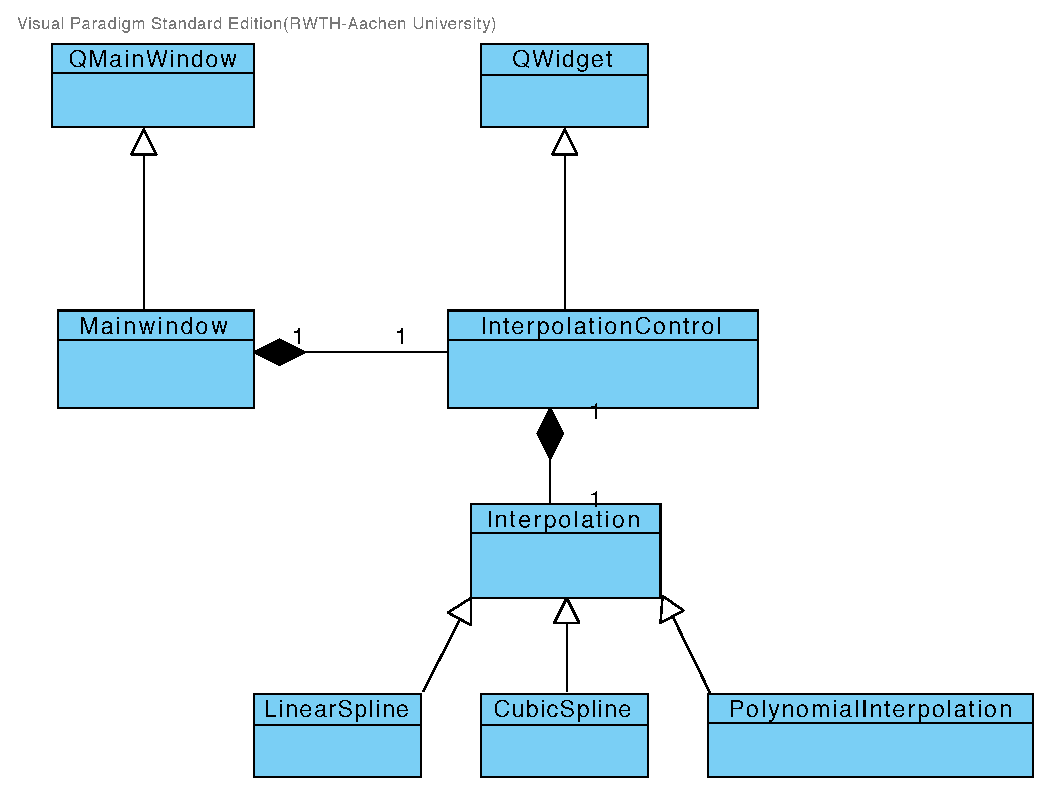
\includegraphics[width=\textwidth]{figures/Begriffsmodel.eps}
\caption{Begriffsmodell}
\end{figure}
